
\section{Tabeller}

\begin{center}
	\begin{tabular}{| m{4cm} |m{4cm} |m{4cm} |} 
\hline
	\multicolumn{3}{|c|}{\textbf{\cellcolor[HTML]{D5D5D5}Oversikt over laboppgaver}} \\
\hline
\hline
\rowcolor [HTML]{D5D5D5}
Finn eller beregn 		&Verdi				&Kommentar							\\ \cline{1-3}
Ib - belastningsstrøm		&				&								\\ \cline{1-3}
In – Nominell størrelse vern	&				&Ib<In								\\ \cline{1-3}
Karakteristikk			&				&								\\ \cline{1-3}
Referanseinstallasjonsmetode	&				&Figur D.1 side 118						\\ \cline{1-3}
2- eller 3-leder		&				&								\\ \cline{1-3}
PVC eller PEX			&				&								\\ \cline{1-3}
Strømføringsevne (Iz) 		&				&Tabell 6 side 81						\\ \cline{1-3}
Tverrsnitt			&				&								\\ \cline{1-3}
Omgivelsestemperatur		&$Temp:	k_temp:$		&Tabell D.1 side 117						\\ \cline{1-3}
Nærføring			&$Antall:	k_ner:$		&Tabell D.2 side 119						\\ \cline{1-3}
Ny Strømføringsevne (Iz)	&$Iz\cdot k_temp \cdot k_ner$ 	&								\\ \cline{1-3}
Krav 1				&				&$Ib<In<Iz$							\\ \cline{1-3}
Krav 2				&				&$I2<1,45 \cdot Iz$						\\ \cline{1-3}
Motstand leder (Rl) 		&				&$Rl= \frac {\rho \cdot l \cdot \sqrt{3} \cdot cos\phi}{A}$ 	\\ \cline{1-3}
Motstand ved 70°C ($Rl_{70}$)	&				&$Rl_70=Rl \cdot 1,2$						\\ \cline{1-3}
Spenningsfall $\Delta U$	&				&$\Delta U=Rl_70 \cdot Ib$					\\ \cline{1-3}
Spenningsfall \%  		&				&$\Delta Ui \%=  \Delta U/U*100\%$				\\ \cline{1-3}
Vurdering spenningsfall 	&				&								\\ \cline{1-3}
Kontroller at vernet ikke slår ut på startstrømmen 	& 				&I_start< I_4 							\\ \cline{1-3}
Ikmin på siste punkt		& 				&								\\ \cline{1-3}
Vernets I5			& 				&								\\ \cline{1-3}
Løser vernet ut momentant ved kortslutning 			& 				&I_5≤〖Ik〗_min 						\\ \cline{1-3}
Hvor lang tid tar det før vernet løser ut			& 				& 								\\ \cline{1-3}
Kontroller maksimal kabellengde &				&Tabell 10 side 102 						\\ \cline{1-3}
Tåler vernet største kortslutning 			& 				&Ik_maks≤I_cu 							\\ \cline{1-3}
Hvor lenge tåler kabelen kortslutningen  		& 				&D.4 side 121  t=(k*S/I)^2 					\\ \cline{1-3}
Løser sikringen ut før kabelen blir ødelagt? 			& 				&0,1s < t < 5s 							\\ \cline{1-3}


		
\end{tabular}
\end{center}



	
\newpage
\includegraphics[width=1\textwidth]{002.eps}
\vfil \eject
\includegraphics[angle=90,height=1\textheight]{./chemistry12.eps}
\vfil \eject
\includegraphics[width=1\textwidth]{calibrate03.eps}
\includegraphics[width=1\textwidth]{calibrate04.eps}
\includegraphics[width=0.5\textwidth]{current09.eps}
\includegraphics[width=0.5\textwidth]{current10.eps}
\includegraphics[width=0.5\textwidth]{current11.eps}
\includegraphics[width=0.5\textwidth]{current12.eps}
\includegraphics[width=0.5\textwidth]{current13.eps}
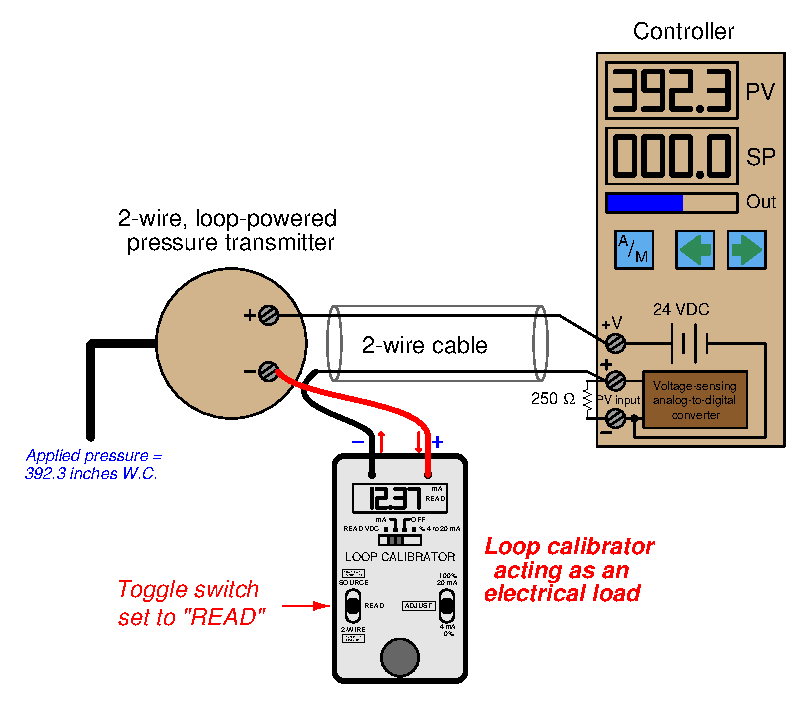
\includegraphics[width=0.5\textwidth]{current29.eps}
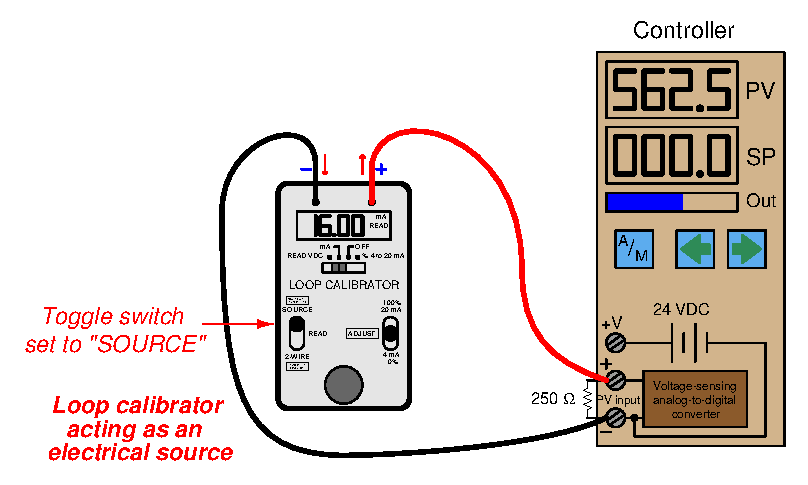
\includegraphics[width=0.5\textwidth]{current30.eps}
\includegraphics[width=0.5\textwidth]{current31.eps}
\includegraphics[width=1\textwidth]{plc_048.eps}
\includegraphics[width=1\textwidth]{plc_052.eps}
\includegraphics[width=1\textwidth]{pressure76.eps}
